% ============================================================
%  SCHOLA DOMESTICA — Level 1, Week 1, Lesson 4
%  Topic: Comparing Groups — More, Fewer, Same (Numbers 1–5)
% ============================================================
% Save as: sd_L1_W1_L4.tex

\documentclass[12pt,letterpaper]{article}
\usepackage[top=1in,bottom=1in,left=1in,right=1in]{geometry}
\usepackage{fontspec}\usepackage{graphicx}\usepackage{xcolor}
\usepackage{mdframed}\usepackage{tikz}\usepackage{fancyhdr}\usepackage{parskip}
\usetikzlibrary{shapes.geometric}
\setmainfont{EB Garamond}[Ligatures=TeX,Numbers=OldStyle]
\definecolor{sd-blue}{RGB}{60,100,160}\definecolor{sd-gold}{RGB}{180,140,50}
\definecolor{sd-light}{RGB}{245,242,235}\definecolor{sd-green}{RGB}{70,130,80}
\pagestyle{fancy}\fancyhf{}
\fancyhead[L]{\small\color{sd-blue}\textit{Schola Domestica Mathematics}}
\fancyhead[R]{\small\color{sd-blue}\textit{Level~1 \(\cdot\) Week~1 \(\cdot\) Lesson~4}}
\fancyfoot[C]{\small\color{sd-blue}1}
\renewcommand{\headrulewidth}{0.4pt}
\newmdenv[backgroundcolor=sd-light,linecolor=sd-blue,linewidth=1pt,
  innerleftmargin=10pt,innerrightmargin=10pt,innertopmargin=8pt,
  innerbottommargin=8pt,roundcorner=4pt]{instructbox}
\newmdenv[backgroundcolor=white,linecolor=sd-green,linewidth=1.5pt,
  innerleftmargin=10pt,innerrightmargin=10pt,innertopmargin=8pt,
  innerbottommargin=8pt,roundcorner=4pt]{checkbox}
\newcommand{\ansblank}{\underline{\hspace{1.8cm}}}
\newcounter{probnum}
\newcommand{\prob}{\stepcounter{probnum}\noindent\textbf{\arabic{probnum}.}\quad}
\newcommand{\onestar}{
\begin{tikzpicture}[baseline=-0.1cm]
  \node[star,star points=5,star point ratio=2.5,fill=sd-gold,
        draw=sd-gold!80!black,minimum size=0.9cm]{};
  \end{tikzpicture}}
\begin{document}
\begin{center}
  {\color{sd-blue}\Large\bfseries Schola Domestica Mathematics — Level~1}\\[4pt]
  {\color{sd-blue}\rule{\linewidth}{1.5pt}}\\[6pt]
  {\LARGE\bfseries Lesson 4 \quad|\quad More, Fewer, or the Same?}\\[4pt]
  {\color{sd-gold}\rule{\linewidth}{0.8pt}}
\end{center}
\vspace{4pt}
\begin{instructbox}
\noindent\textbf{\color{sd-blue}Instruction:}\\[4pt]
When one group has more objects than another, we say it has \textbf{more}.
When it has fewer, we say \textbf{fewer}.
When they match exactly, we say \textbf{same}.
\end{instructbox}
\vspace{8pt}
\noindent\textbf{\color{sd-blue}Practice}
\vspace{6pt}

\prob Which group has \textbf{more}? Circle it.\\[4pt]
\begin{tabular}{lcl}
Group A: & \onestar\onestar\onestar & (3 stars)\\[4pt]
Group B: & \onestar\onestar\onestar\onestar\onestar & (5 stars)
\end{tabular}

\vspace{10pt}
\prob Which group has \textbf{fewer}? Circle it.\\[4pt]
\begin{tabular}{lcl}
Group A: &
\IfFileExists{apples_4.jpg}{
\includegraphics[height=1.3cm]{apples_4.jpg}}{%
  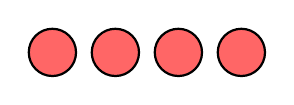
\begin{tikzpicture}[baseline=0]\foreach\x in{0,1,2,3}\draw[fill=red!60,thick](\x*0.8,0)circle(0.3);\end{tikzpicture}}
& (4 apples)\\[4pt]
Group B: &
\IfFileExists{apples_2.jpg}{
\includegraphics[height=1.3cm]{apples_2.jpg}}{%
  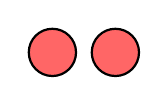
\begin{tikzpicture}[baseline=0]\foreach\x in{0,1}\draw[fill=red!60,thick](\x*0.8,0)circle(0.3);\end{tikzpicture}}
& (2 apples)
\end{tabular}

\vspace{10pt}
\prob Are these groups the \textbf{same}? Write yes or no.\\[4pt]
\begin{tabular}{lcl}
Group A: & \onestar\onestar\onestar & \\[4pt]
Group B: & \onestar\onestar\onestar &
\end{tabular}\quad\ansblank

\vspace{10pt}
\prob Draw a group with the \textbf{same} number as these ducks:\\[4pt]
\IfFileExists{ducks_4.jpg}{
\includegraphics[height=1.6cm]{ducks_4.jpg}}{%
  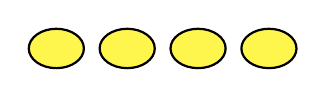
\begin{tikzpicture}[baseline=0]\foreach\x in{0,1,2,3}\draw[fill=yellow!70,thick](\x*0.9,0)ellipse(0.35 and 0.25);\end{tikzpicture}}\\[6pt]
\noindent\fbox{\rule{0pt}{2.2cm}\hspace{9cm}}

\vspace{10pt}
\prob \textit{(Teacher reads)} A pond has 3 goldfish. A bowl has 5 goldfish.
Which has more? \quad\ansblank

\vspace{10pt}
\prob Write the number that is \textbf{more}: \quad 2 \quad or \quad 4 \quad $\longrightarrow$ \quad\ansblank

\vspace{10pt}
\prob Write the number that is \textbf{fewer}: \quad 5 \quad or \quad 3 \quad $\longrightarrow$ \quad\ansblank

\vspace{10pt}
\prob \textit{(Teacher reads)} Sara has 2 flowers. Tom has 2 flowers.
Do they have the same? \quad\ansblank

\vspace{8pt}{\color{sd-gold}\rule{\linewidth}{0.5pt}}\vspace{4pt}
\begin{checkbox}
\noindent\textbf{\color{sd-green}Knowledge Check}\\[4pt]
\setcounter{probnum}{0}
\prob Which is more: 3 or 5? \quad\ansblank\\[8pt]
\prob Which is fewer: 4 or 1? \quad\ansblank
\end{checkbox}
\vfill
\noindent{\color{sd-blue}$\bigstar$ \textbf{Enrichment:}}
In Latin: \textit{plus} means more and \textit{minus} means less (fewer).
You already know two math words in Latin!
\vspace{4pt}\hrule\vspace{2pt}
{\footnotesize\color{gray}\textit{Teacher note: Use physical objects to compare groups before the worksheet if the concept is new.}}
\end{document}
